\subsection{Affine Edwards curves}

Let $k$ be an arbitrary field (for simplicity we assumed $k = \mathbb{R}$ in our proof). We define an Edward curve $E$ as the set of zeros of the following multivariate polynomial:

$$e(x,y) = x^2 + cy^2 - 1 - d x^2y^2$$

where $c,d,x,y \in k$ and $c,d$ are fixed. Then one defines the addition of two points on the curve as:

$$z_1 \oplus z_2 = (x_1,y_1) \oplus (x_2,y_2) = \Big(\frac{x_1x_2-cy_1y_2}{1-dx_1x_2y_1y_1},\frac{x_1y_2+y_1 y_2}{1+d x_1 x_2 y_1y_2}\Big)$$

The motivation for this addition is explained in \cite{hales2016group} in a very accessible manner without going into the details of algebraic geometry. Essentially, one reinterprets the normal complex multiplication:

$$(x_1,y_1) \cdot (x_2,y_2) = (x_1 x_2 - y_1 y_2, x_1 y_2 + x_2 y_1)$$

by considering the family of hyperbolas in the plane that pass through $z = (-1,0)$ and whose asymptotes are parallel to the coordinate axes, these are given by the equation:

$$xy + p(x + 1) + qy = 0$$

Every two points $z_1$ and $z_2$ on the circle intersect some hyperbola within the family. The hyperbola meets the unit circle in one additional point $z_3$:

\begin{center}
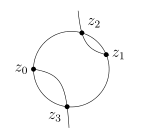
\includegraphics{img/hyp_circ.png}
\end{center}

It turns out that $z_1 z_2 z_3 = 1$ and one may define complex multiplication as $z_1 z_2 = \overline{z_3}$. The very same construction works for general elliptic curves and gives the addition formula above:

\begin{center}
	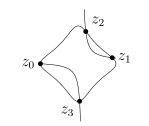
\includegraphics{img/hyp_ellip.png}
\end{center}

The goal of \cite{hales2016group} is to show that $(E,\oplus)$ is an abelian group. This is only feasible for affine Edwards curves when $d$ is not a non-null square.

\subsection{Projective Edwards curves}

Introduced to bypass the restriction that $d$ should not be a non-null square. 

Introduced by gluing two affine curves $E_{\text{aff}}$ together. 

The associative property for $E$ is a direct consequence of the associative property of the affine pieces $E_{\text{aff}}$.

More formally, one introduces the set $E_{\text{aff}}$ as the set of zeros of the equation:

$$e(x,y) = x^2 + y^2 - 1 - t^2 x^2 y^2$$

One also denotes by $E_{\text{circ}}$ the subset $E_{\text{aff}}$ whose coordinates $x,y$ are non-zero. Finally, in the cartesian product $E_{\text{aff}} \times E_{\text{aff}}$ we use the notation $(P,i)$ to refer to point $P$ of $E$ using the $i$-th copy of $E_{\text{aff}}$ and we identify over the elements of $E_{\text{circ}}$ the pair of points $(P,i)$ and $(\tau P, i+1)$. So elements of $E$ are actually classes of points that we denote by $[P,i]$.

The addition on $E$ requires first to define a second addition $\oplus_1$ (previous addition is denoted from now on by $\oplus_0$) given by:

$$z_1 \oplus_1 z_2 = (x_1,y_1) \oplus_1 (x_2,y_2) = \Big(\frac{x_1y_1-x_2y_2}{x_2y_1 - x_1y_2},\frac{x_1y_1+x_2 y_2}{x_1 x_2 + y_1y_2}\Big)$$

Finally, addition on $E$ is defined by:

$$[P,i] \oplus [Q,j] = [P \oplus_l Q, i+j]$$

if $\delta_l(P,Q) \neq 0, l \in \mathbb{F}_2 = \{0,1\}$ where $\delta_l$ is the magnitude ensuring that the quotients are non-zero. Here, one still needs to prove that $\oplus$ is well-defined. Well-definition and an auxiliary lemma called dichotomy are actually the hardest properties to be established in the development. 

\subsection{Use of Edwards curves}

Edwards curves present several advantages compared to traditional Weierstrass form. To start with, they lead to an explicit formula for addition while in Weierstrass curves addition needs to take care of the special \textit{infinity point}. Also, Bernstein and Lange \cite{bernstein2007faster} showed that addition and multiplication by scalars could be done more efficiently over these curves. Another strong property noted in this study is that if $d$ is not a square the addition was defined for all input pairs on the curve. This is the so-called completeness property of addition. Essentially, it tells that the Edwards addition law can carry out any sequence of group operations, without risk of failure \cite{bernstein2007faster}.

Furthermore, there are important issues arising from the implementation of elliptic curves that should be kept in mind. Literature has given special attention to the so-called side-channel attacks. These cryptographic attacks are based in the measurement of the physical parameters of the system. For instance, one could measure the power consumption \cite{kocher1999differential} or the time spent in executing the underlying algorithm \cite{kasper2011fast} in order to gain information on the cryptographic parameters used. Edwards curves seem to be useful to prevent this kind of attacks \cite{bernstein2007faster}.  

As for projective Edwards curves, which are known in the literature as twisted Edwards curves, they provide a generalization of affine Edwards curves covering a wider range of algebraic curves (in particular, the important class of Montgomery curves) which leads to faster arithmetic computations. The advantage of formalizing this curves lies in the fact that we do not special conditions on the defining parameters to get a group law with their addition \cite{bernstein2008twisted}. 


All of these properties made Edwards curves and their extensions to be of interest in the field of elliptic curve cryptography. 



